This chapter presents the results achieved by the chosen methods introduced in Chapter \ref{section::methodology}. The results achieved by each method are collected under the following subchapters respectively. This chapter provides answers to RQ2 and RQ3 (Chapter \ref{section::introduction}).

\subsection{Exploratory Data Analysis}
    % unique voters
    By the end of 2017, there is a total number of 573 contests in the platform. To identify what kind of content that is more engaging (RQ2), first let us look at the amount of unique voters over the number of contests. Figure \ref{user_engagement_in_contests} displays a histogram and a boxplot of the number of contests and the number of unique voters that they have engaged. 
    
    \begin{figure}[h] 
        \begin{center}
            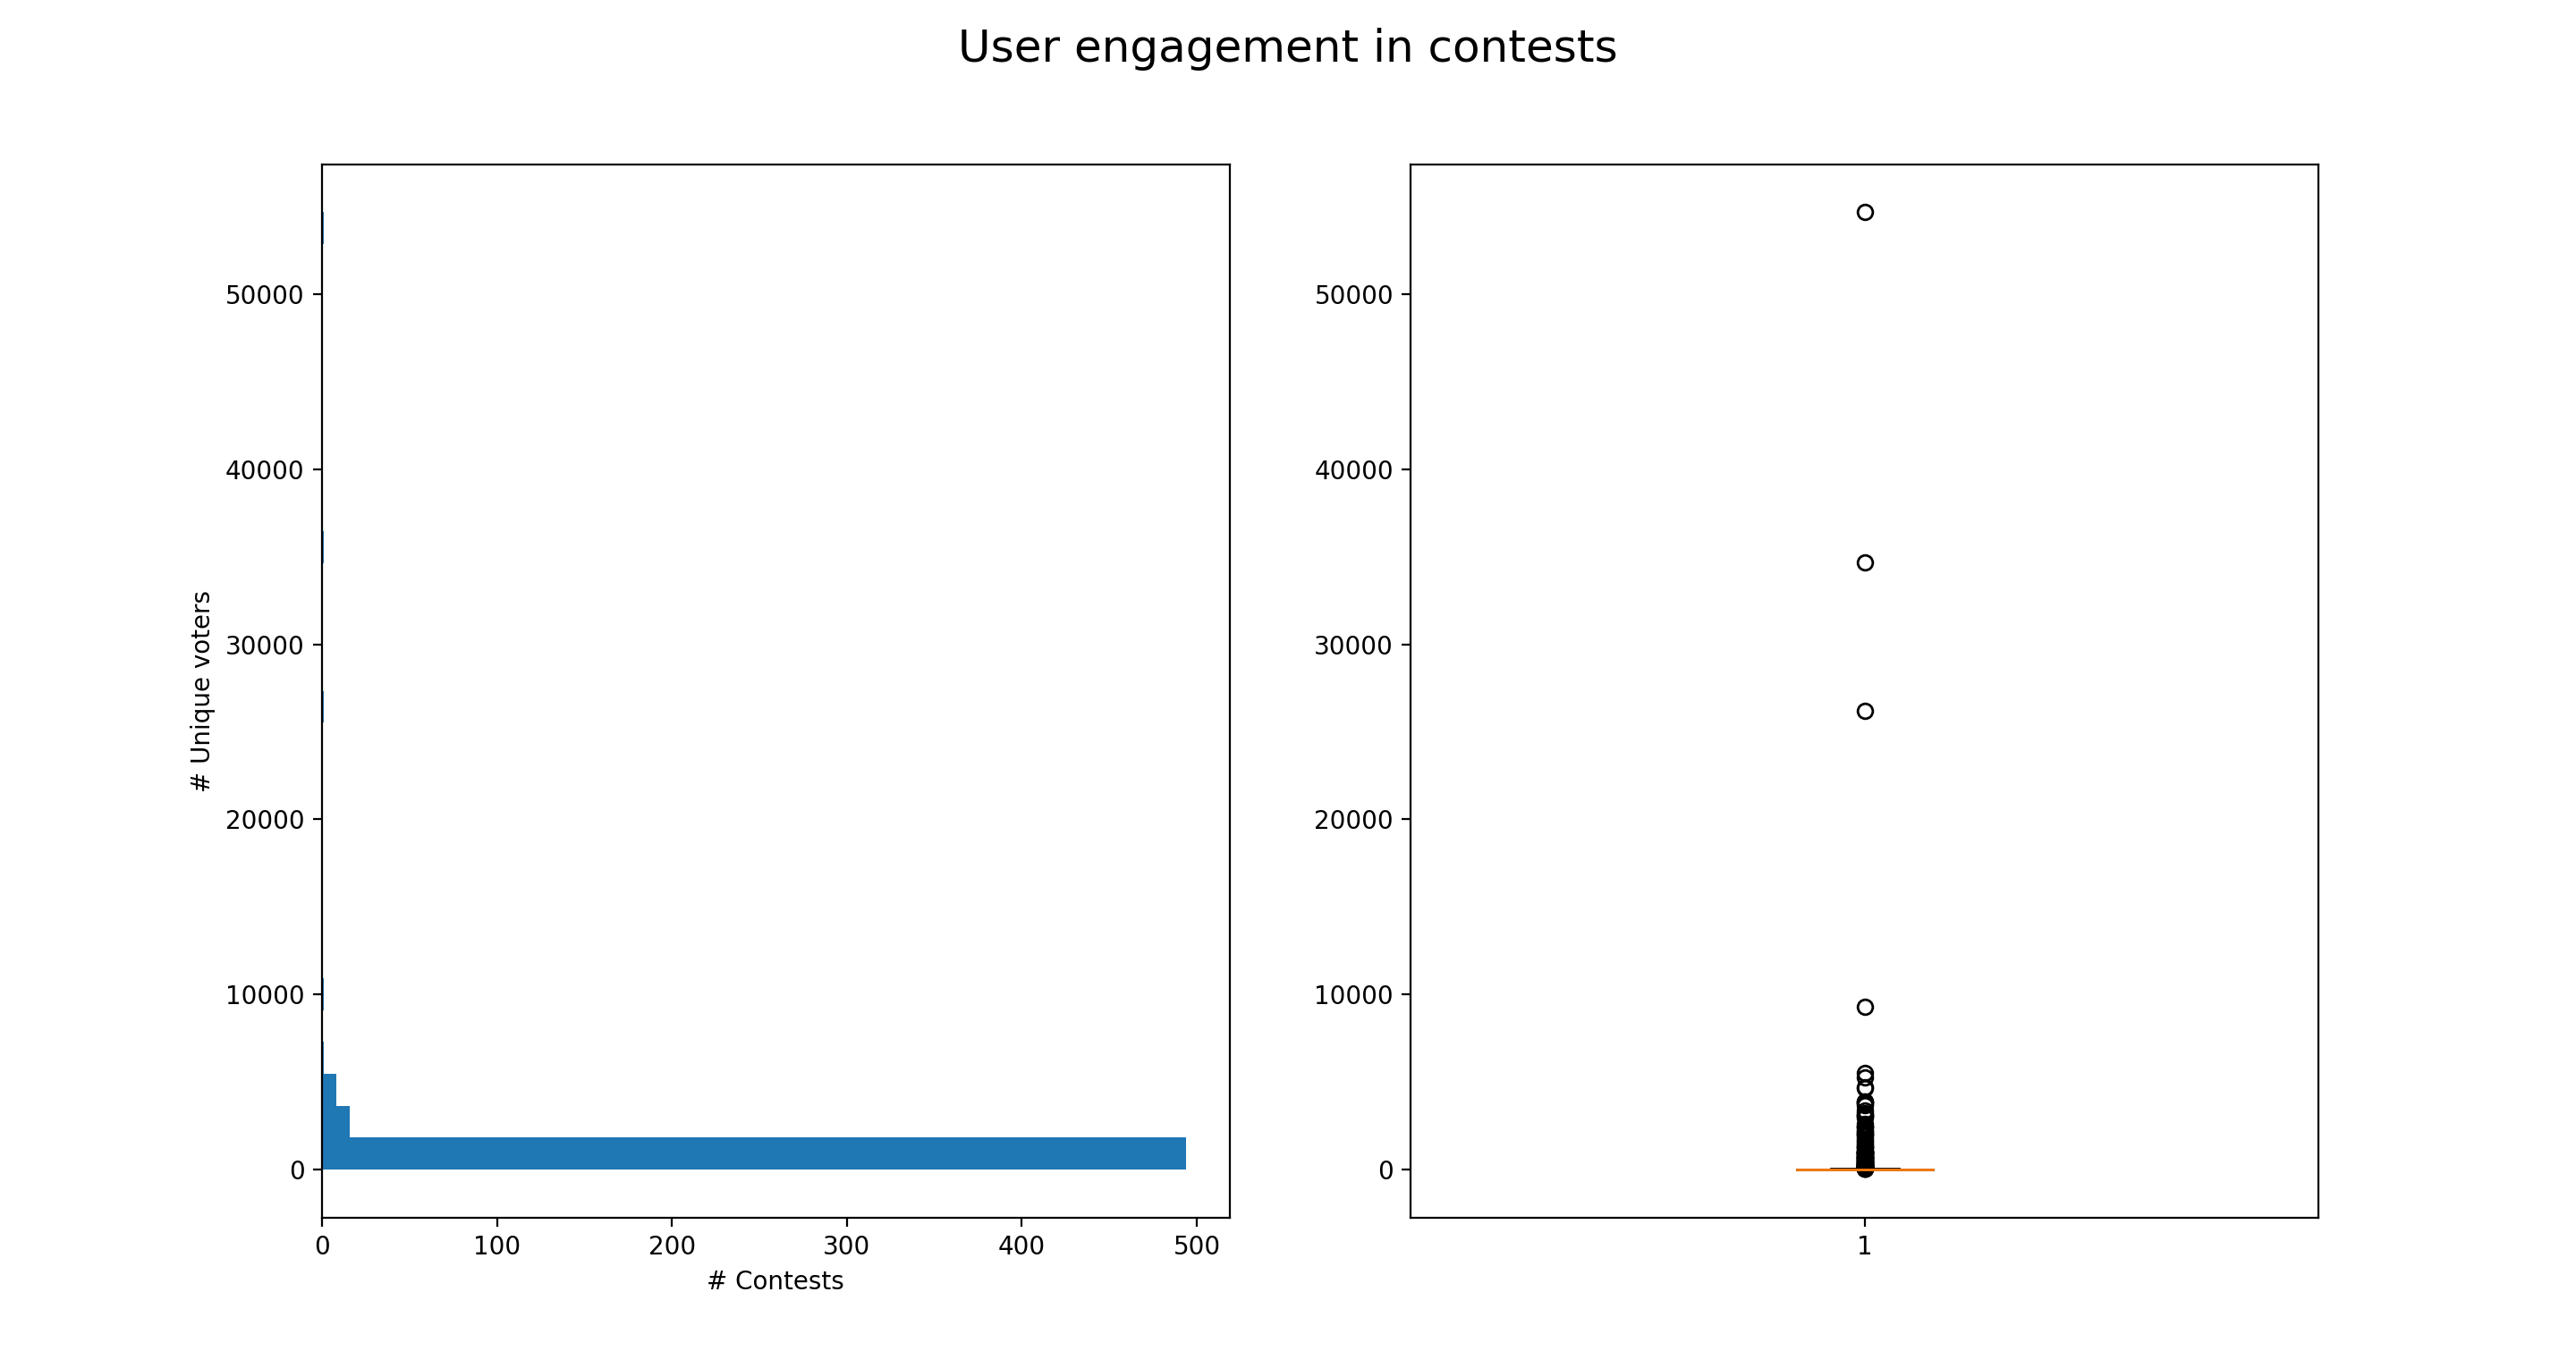
\includegraphics[width=0.8\textwidth]{Images/user_engagement_in_contests.png}
            \caption{The number of unique voters over contests.}
            \label{user_engagement_in_contests}
        \end{center}
    \end{figure}

    It can be easily seen that most of the contests engage very small amount of users, as the median of the unique voter count for all contests is 3. One of the reasons behind this is that the company did not establish a large user base yet. Therefore there are many users who created only one contest but never used the platform on the long run. Many of the contests serve only testing purposes, hence engage only a few users. Such records can create bias in the upcoming analyses, because their data does not represent realistic scenarios. For this reason, contests with less than $100$ unique voters are excluded in the remainder of the analysis, because such observations are not representative. For the remainder of the analyses, this filtered dataset is used.

    Figure \ref{user_engagement_in_contests-pruned} displays the same distribution for the filtered set of contests. In this figure contests with more voters are more apparent. The highest number of unique voters is close to $55 000$ in one of the contests, the mean value ($\mu = 455.43$) and the standard deviation ($\sigma = 3 017.51$). These numbers mean that there is a large variance in the amount of engaged users in contests. It cannot be clearly said which traits make a contest more attractive to users.
    
    The boxplot on the right side of the figure uses the $95$ percentile (around $5 200$ unique voters), above which the outliers can be seen. It can be also seen that the most of the contests engage $260-2 600$ unique voters (as described by the first and the third quartiles). There are $6$ large contests, from which the biggest have engaged $54 684$ voters. 

    \begin{figure}[h] 
        \begin{center}
            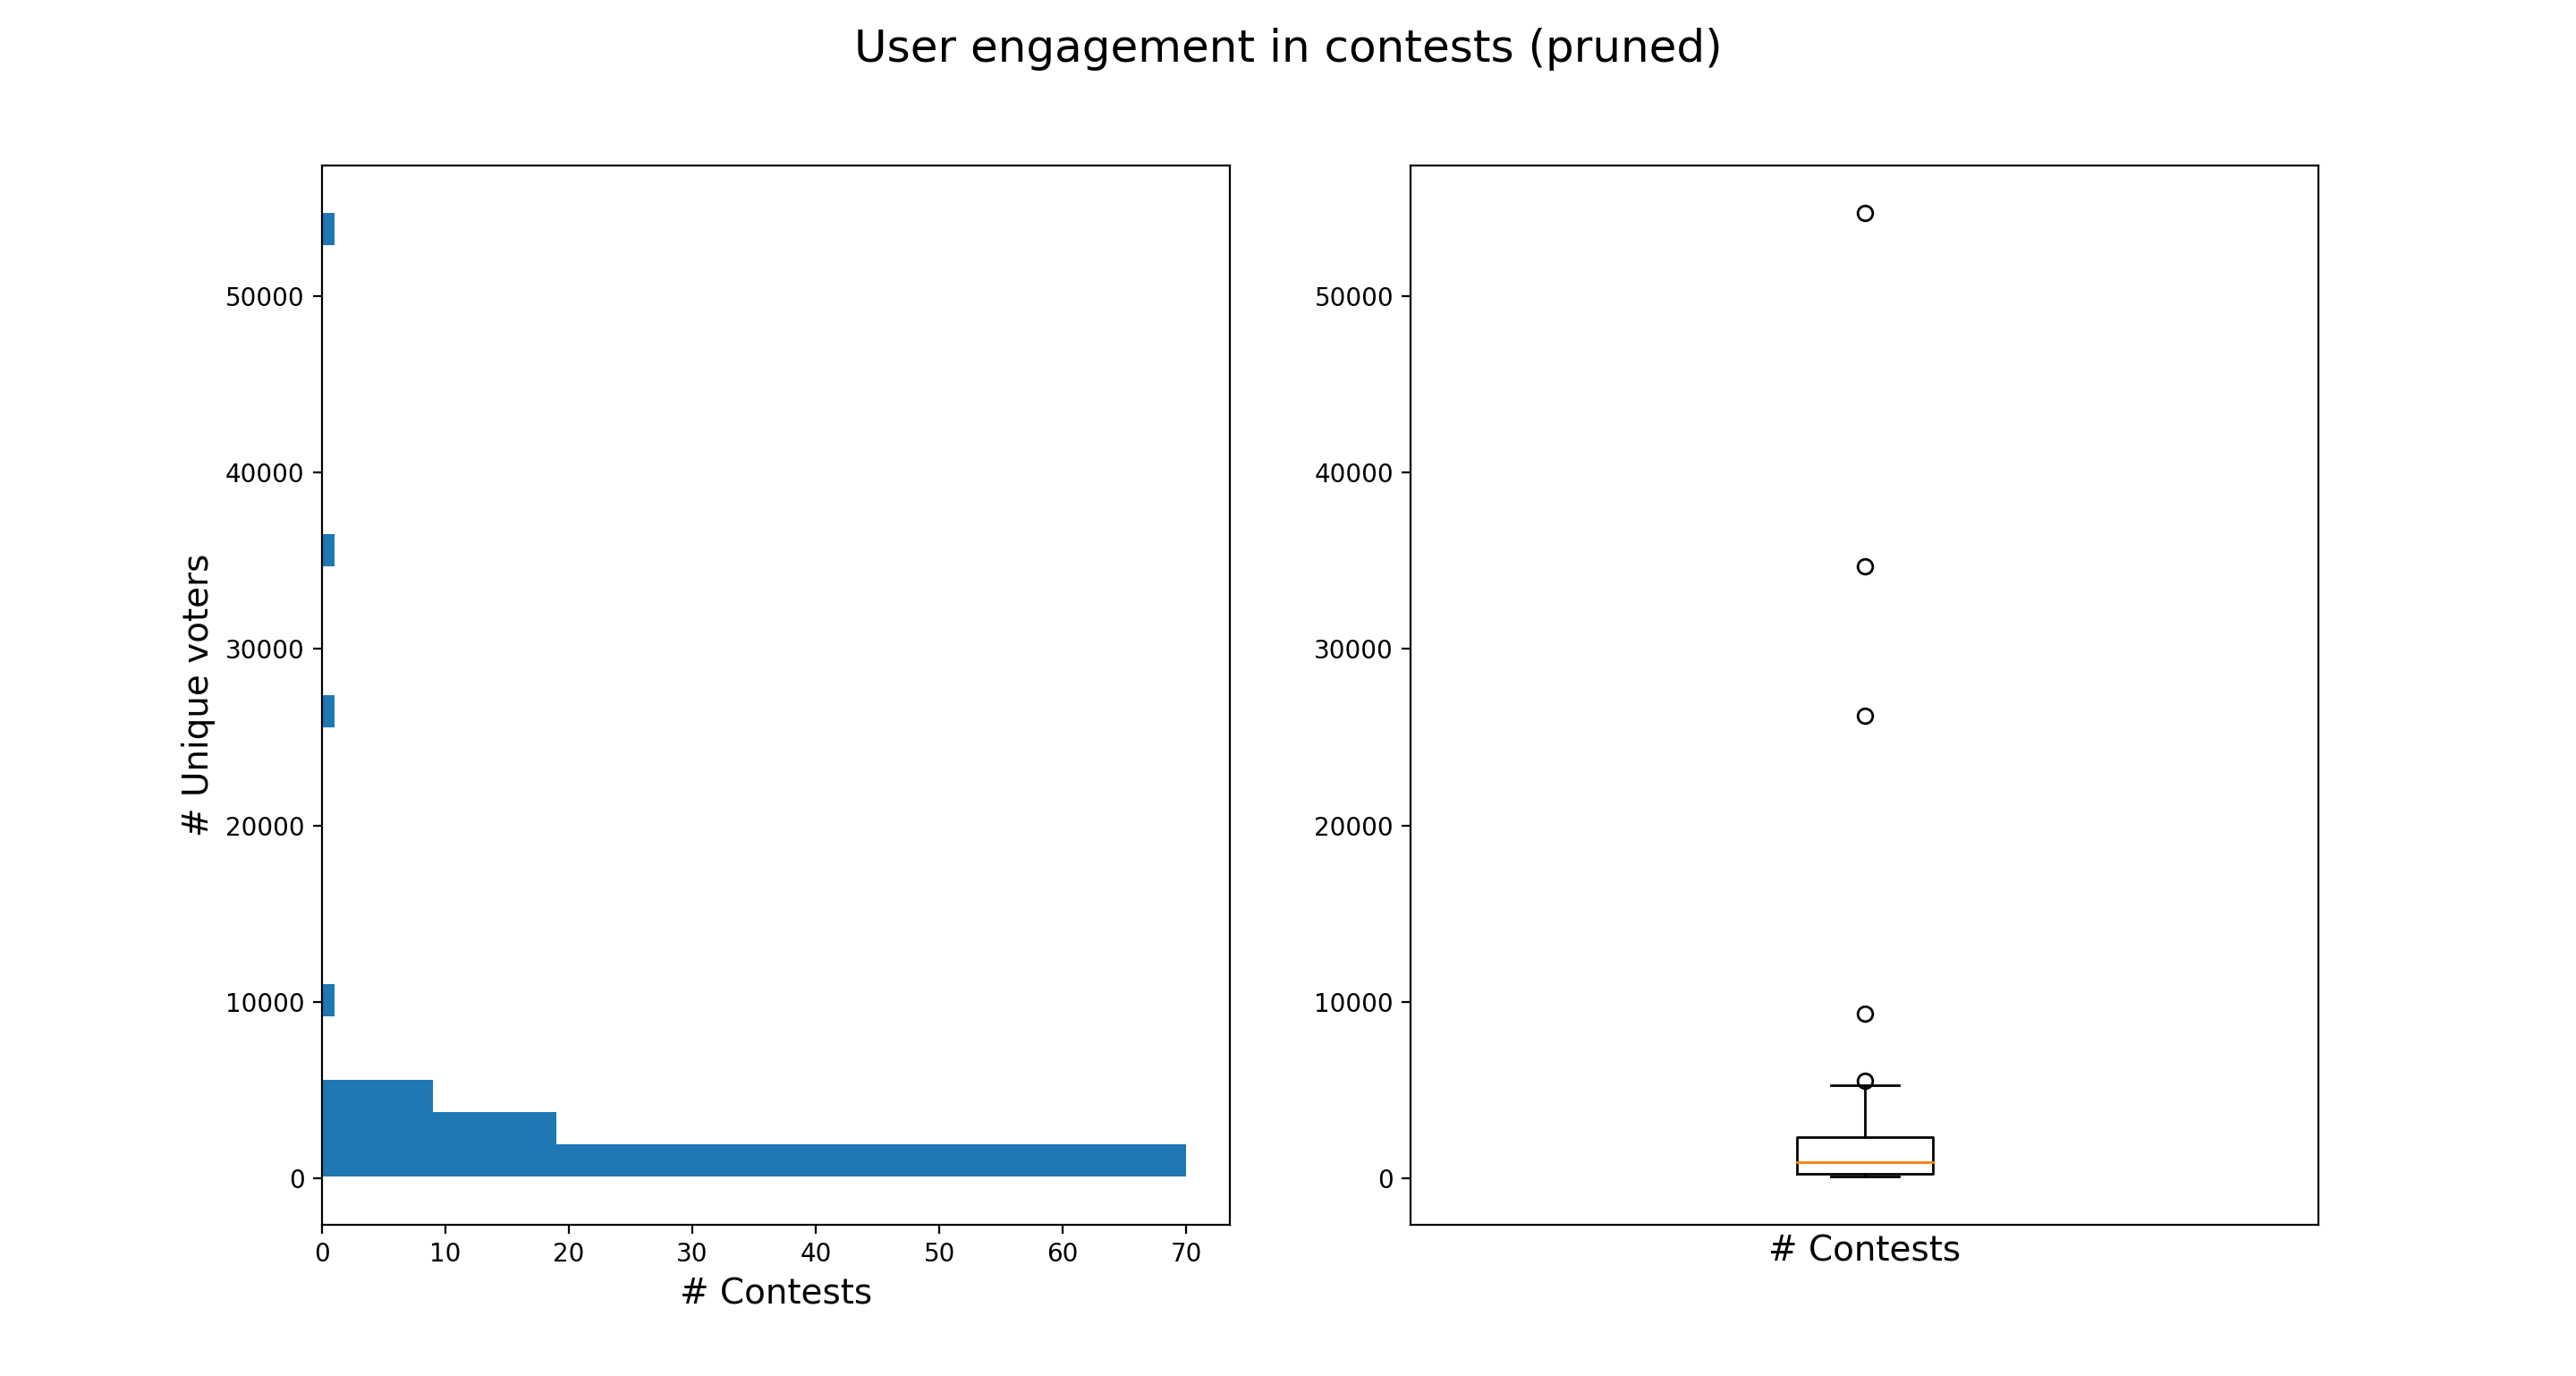
\includegraphics[width=0.8\textwidth]{Images/user_engagement_in_contests-pruned.png}
            \caption{The number of unique voters over contests after filtering out contests with less than $100$ unique voters.}
            \label{user_engagement_in_contests-pruned}
        \end{center}
    \end{figure}
    
    The six large contests are worth investigating a bit more closely. Four \footnote{\url{https://choicely.com/contest/5ca98554-0f7d-11e7-9f0c-6f102a54d68d}}\footnote{\url{https://choicely.com/contest/fb112461-9000-11e6-9e28-87ebd7a21d0d}}\footnote{\url{https://choicely.com/contest/7425566e-8c8e-11e6-b8ce-2147b021362f}}\footnote{\url{https://choicely.com/contest/164f52c7-9df8-11e7-b3c9-d1a0f88250ad}}
    out of the six large contests were beauty pageants, labeled with the categories of "beauty", "fashion" and "entertainment". The two other contests
        \footnote{\url{https://choicely.com/contest/50819173-f838-11e6-b171-b949f18a4d21}}
        \footnote{\url{https://choicely.com/contest/4257ea9c-3e21-11e7-84ec-5f5a9bcfd190}}
    are listed only in the "other" category, which is certainly a mistake. By looking at the latter two contests, it can be easily seen that they would better belong to the "entertainment" and "sports" category. In each of the contests, the contest participants were people: either sportsmen, celebrities or beauty queens/kings. It is interesting that none of the large contests have had objects, places or other intangibles as contest participants, although the platform has seen many of such participants previously. The number of participant in these contests varies between $9-40$ and their correlation coefficient does not show strong relationship either way ($R = 0.53$). 

    In the next step, let us look at the distribution of contest categories in the filtered set of contests. It can be seen from the histogram on Figure \ref{contests_over_categories}, that the amount of "beauty", "entertainment", "sport" and "fashion" contests is considerably high compared to the rest of the categories. This finding is well aligned with the case company's profile at the point of conducting this study. As pointed out in Chapter \ref{section::introduction-to-the-choicely-voting-platform}, most of the company's customer base consits of Finnish broadcasters and advertisers. Hence there is no surprise in the distribution of the categories except for the "other" group. 
    
    \begin{figure}[h] 
        \begin{center}
            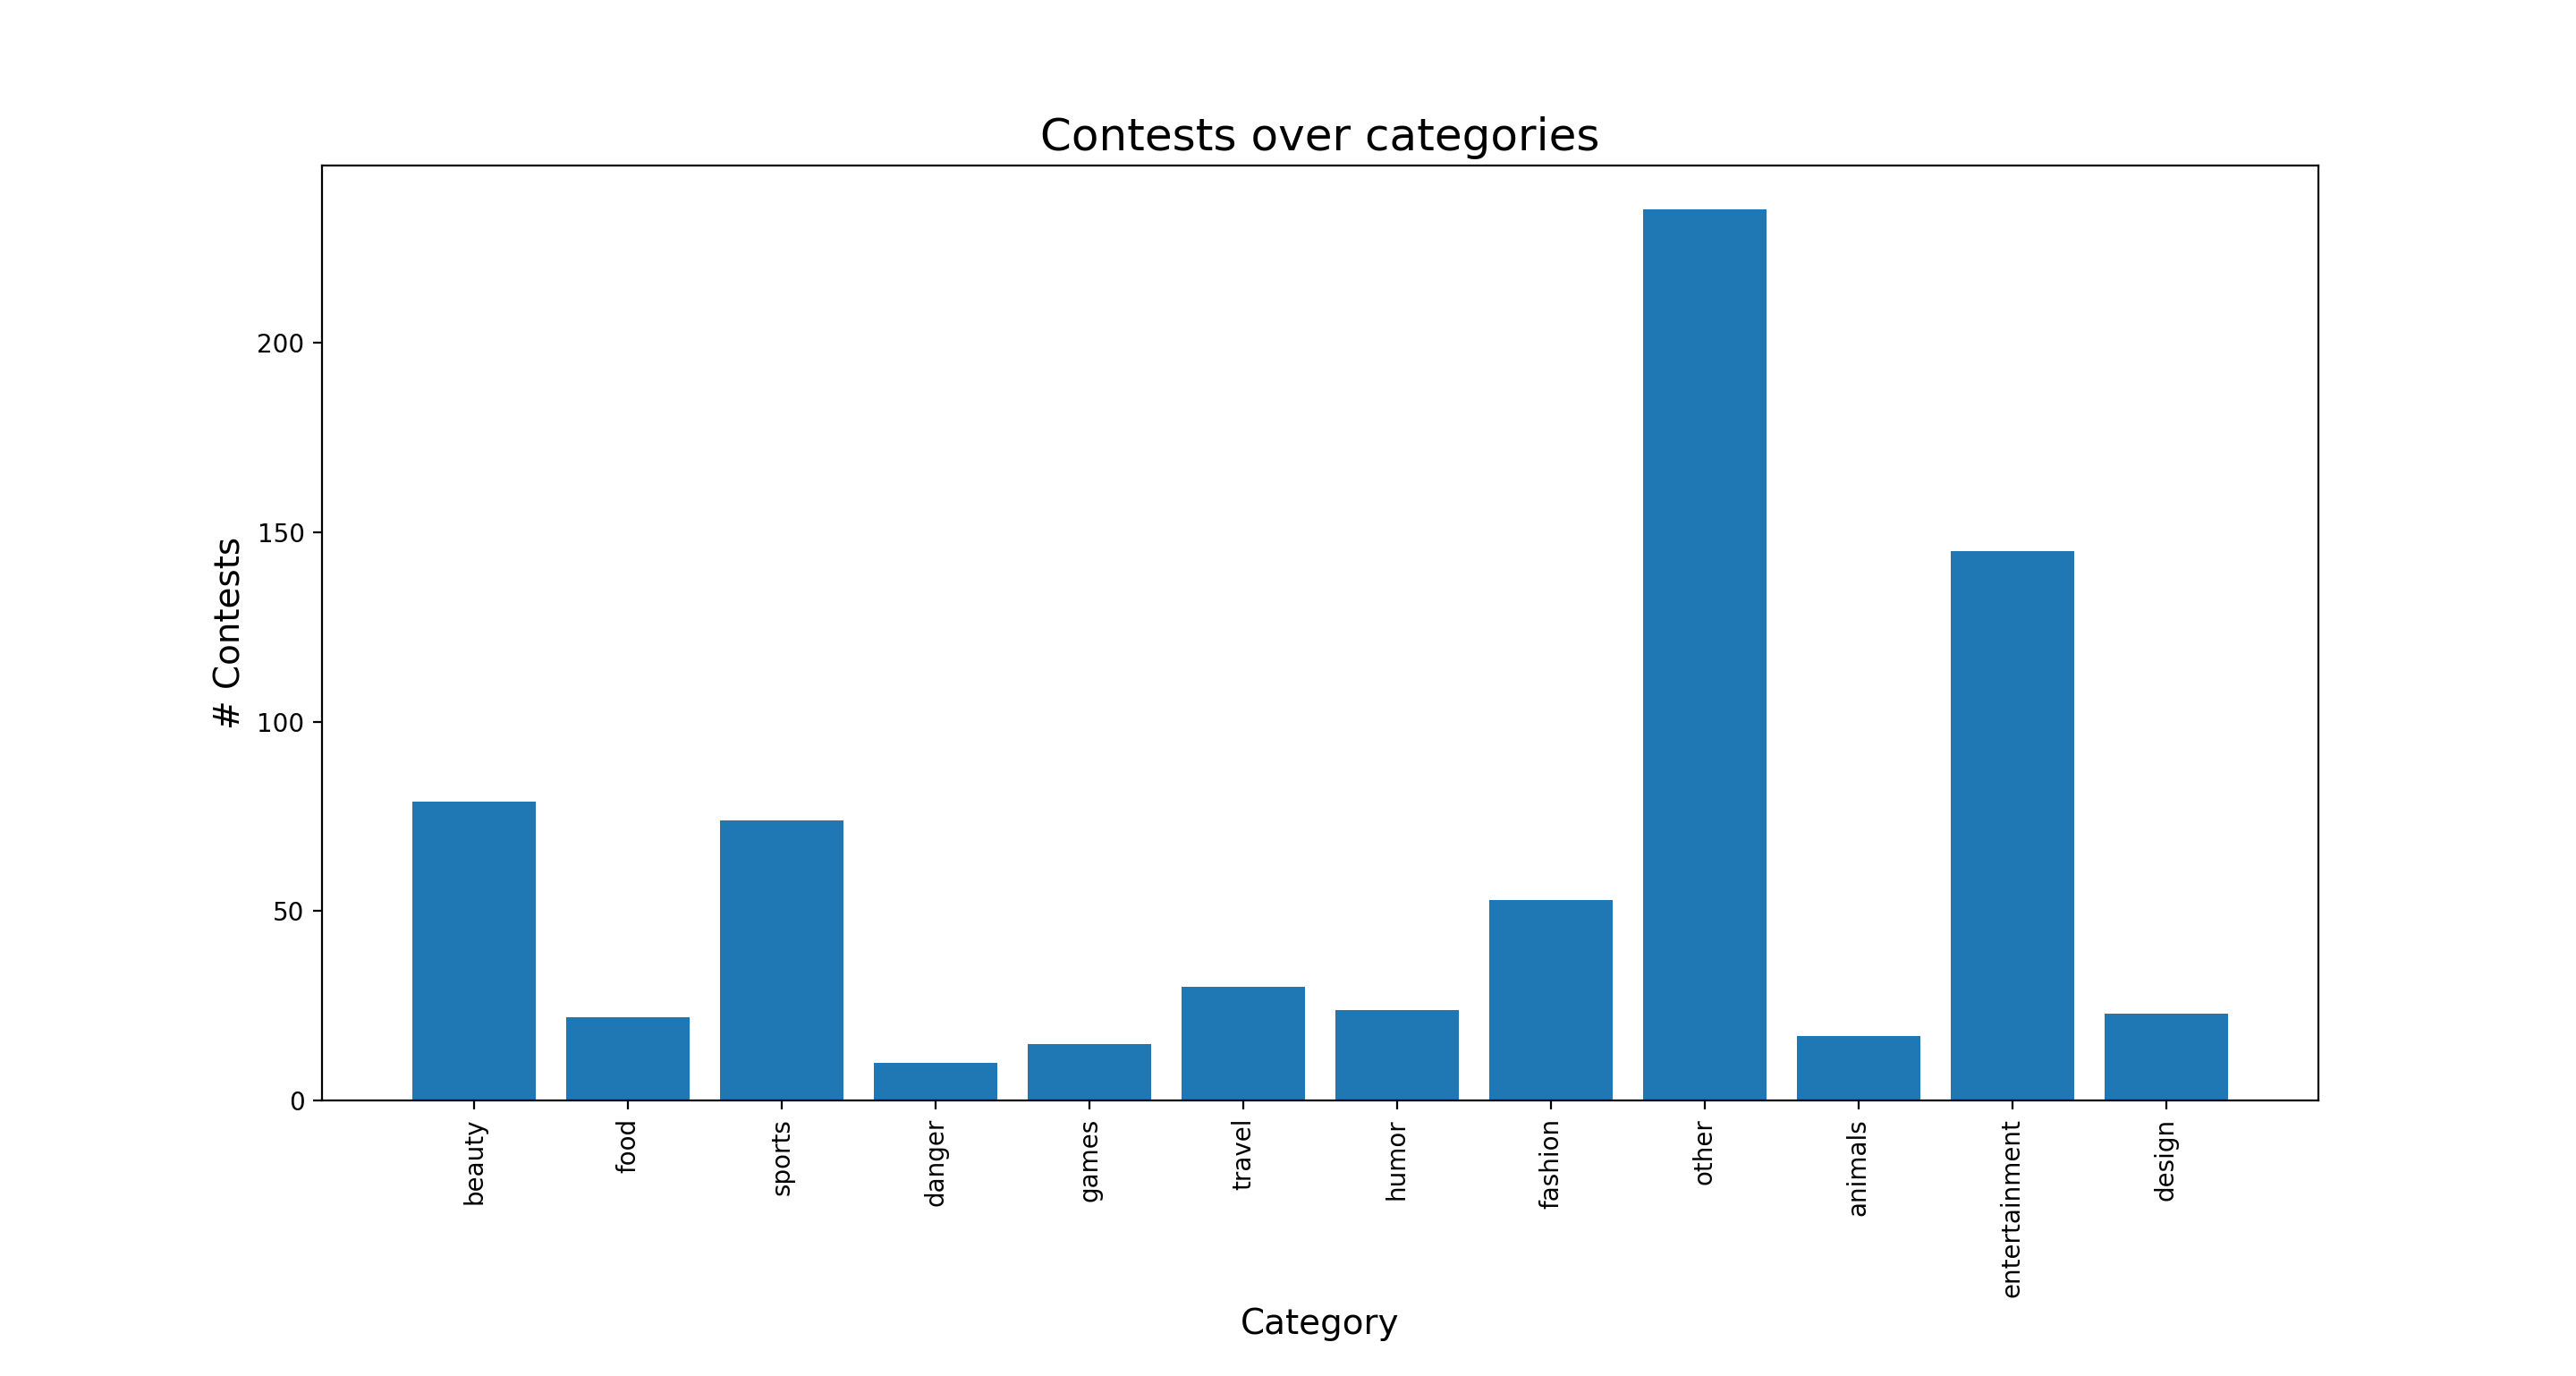
\includegraphics[width=0.8\textwidth]{Images/contests_over_categories.png}
            \caption{The number of contests in each category.}
            \label{contests_over_categories}
        \end{center}
    \end{figure}
    
    By manually looking at contests in the "other" category it can be seen, that many (28 out of 34) of these contests is actually a sport-related. To name a few examples, there are contests with titles as "Best player poll" ("Paras pelejaa aanestys")\footnote{\url{https://choicely.com/contest/5f8f8470-914d-11e6-bd5b-e571d894172f}}, "Who is the hottest driver?" ("Kuka on kuumin kuski?")\footnote{\url{https://choicely.com/contest/93d5f89c-5676-11e7-8cf7-0759c198269e}}, "Fastest driver of the race" ("Kisan nopein kuski")\footnote{\url{https://choicely.com/contest/bb7db707-3683-11e7-9f48-cbe34704f83e}}. This finding is not a suprise knowing the firm's customer base, but it also suggests the popularity of sports contests. If these contests were labelled correctly, sports contest would top the charts (Figure \ref{contests_over_categories}) with the highest bin around 50. Another interesting fact is, that in all of the sports contests, participants are athlethes, hence the images contain human beings as well. 
    
    Moreover, three of the contests were related to the "travel" category, one to "fashion" and "beauty" and one to "entertainment". The error in this case is not as high as with sport contests, however correcting these category labels would facilitate data analysis in the future. For this reason, it is suggested to the company to review such issues, correct them manually and potentially prevent them happening in the future. 
    
    To answer the question of most engaging contest categories, the unique voters over contest categories is studied. Simple statistical measures (sum, mean, median and standard deviation) are calculated for the number of unique voters for each contest category. Table \ref{user_engagement_over_categories} displays the results.
    
    It can be seen, that "entertainment" and "beauty" contests cover the majority the amount of uniuqe voters ($\approx 66.60 \%$ of the total). The values of these categories together are similar with the  "fashion" category. In these categories the mean and the median of the voters is also considerably high, which suggests their attractiveness. However, the high values in the standard deviation of the unique voters indicates the wide spreadness of values around the mean. The relevance of this observation is, that not all contests in these categories engage a large audience necessarily. Thus it can be concluded, that these categories tend to appear together and also attract a larger audience compared to the rest in general. 

    \begin{table}[]
        \centering
        \begin{adjustbox}{width=1\textwidth}
            \begin{tabular}{l|c|c|c|c|c}
                \textbf{Contest category} & \textbf{Sum of unique voters} & \textbf{Mean of unique voters} & \textbf{Median of unique voters} & \textbf{Standard deviation of unique voters} \\
                \hline
                beauty & 135866 & 3996.06 & 1482.00 & 9854.14 \\
                other & 61455 & 1807.50 & 1240.50 & 1831.40 \\
                entertainment & 161233 & 5374.43 & 1728.50 & 11772.68 \\
                sports & 15220 & 634.17 & 299.00 & 757.83 \\
                fashion & 75872 & 4742.00 & 874.00 & 12972.72 \\
                travel & 4451 & 1483.67 & 409.00 & 1719.40 \\
                humor & 1367 & 683.50 & 683.50 & 274.50 \\
                food & 767 & 767.00 & 767.00 & 0.00 \\
                danger & 958 & 958.00 & 958.00 & 0.00 \\
                games & 164 & 164.00 & 164.00 & 0.00
            \end{tabular}
        \end{adjustbox}
        \caption{The basic statistical measures of unique voters for each contest category.}
        \label{user_engagement_over_categories}
    \end{table}
    
    The categories "travel", "humor", "food", "danger" and "games" have hosted only a considerably low number of contests (Figure \ref{contests_over_categories}). Due to the small amount of data, it is difficult to derive any relevant results about the attractiveness of these categories at this point. It is suggested for the company to host and advertise more of these contests so that the public's opinion and engagement can be evaluated in these areas as well.

    % As the last part of the EDA, the attributes of highly rated contestants are investigated. In other words it is studied, what kind of traits make a contest participant more attractive to users. To answer this question, the podium finishers of the six large contests explained above are taken as examples. % TODO consider if needed

    % deriving results
    The above results contribute towards answering RQ2. The results allow to derive the following conclusions: 

    \begin{itemize}
        \item many of the contests are not labeled and hence belong only to the "other" category - fixing these labels manually could contribute towards better results,
        \item the "fashion", "beauty" and "entertainment" categories often appear together in contests,
        \item contests in the "beauty" and "entertainment" categories appear to be engaging to large audiences,
        \item contests where participants are human beings appear to be attractive to users,
        \item there is no correlation between the unique voter count and the number of participants,
        \item the platform has hosted only a few contests in some of the categories and hence it is not possible to derive significant findings about the attractiveness of those contets at the moment.
    \end{itemize}

\subsection{Association analysis}
